\clearpage
\sffamily
{\bfseries\color[rgb]{0.4,0.4,0.4}
Law 4 -- The Players ('Equipment')}
\phantomsection
\addcontentsline{toc}{subsection}{Law 4 -- The Players ('Equipment')}

\bigskip

{\bfseries Safety }

\headlinebox

A player must not use equipment or wear anything that is dangerous to himself or another player (including any kind of jewellery).

\bigskip

{\bfseries The Design of the Robots\simplify{ (new)}}

\headlinebox

Robots participating in the Humanoid League competitions must have a human-like body plan, as shown in Fig. \ref{fig:bodyplan}. They must consist of two legs, two arms, and one head, which are attached to a trunk.

\bigskip

\removed{(new:) Robots in KidSize must be
equipped with a handle, to be picked up safely and with no harm to the robot and
the handler.}


\begin{figure}[h]
\begin{center}
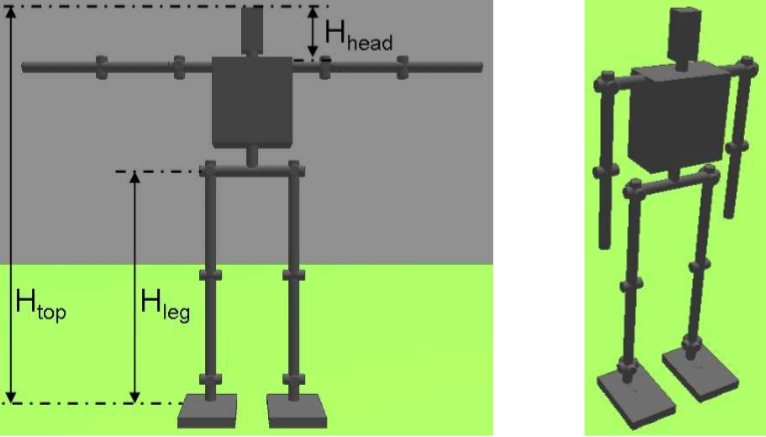
\includegraphics[width=0.7\textwidth]{img/bodyplan.png}
\caption{Example of a humanoid robot body plan (left) and standing upright pose (right)}
\label{fig:bodyplan}
\vspace{-3ex}
\end{center}
\end{figure}


The robots must be able to stand upright on their feet and to walk on their legs.
KidSize robots need to be able to recover from a fall
(get back to a standing position).
The only allowed modes of locomotion are bipedal walking, running and jumping.

\bigskip

All actions of the robots must be kinematically equivalent to humanoid motions.

\bigskip

\removedSection{
\removed{
  Robots must be equipped with an emergency stop button that makes the robot immediately desist with all motions, or ideally go limp and/or cut power to the actuators. In addition to the emergency stop button, robots may only have up to two additional physical or virtual buttons: One to start the robot behaviour and one to stop the behaviour. The buttons must be clearly labeled. If the robot has more buttons that cannot be detached, they must be visibly masked during the games.}

\bigskip
}


\added{Body parts considered as feet and hands must be marked in the robot model.}

\bigskip

{\bfseries Robot Height\simplify{ (new)}}

\headlinebox

Based on $H_{top}$, the following size restrictions apply:

\begin{itemize}
\item 40 cm ${\leq}$ $H_{top}$ ${\leq}$ 100 cm to play in the KidSize class,
\item 100 cm ${\leq}$ $H_{top}$ ${\leq}$ 200 cm to play in the AdultSize class.
\end{itemize}

$H_{top}$ is defined as the height of the robot when standing upright (with fully extended knees, cf. Fig. \ref{fig:bodyplan} right) and $H_{COM}$ denotes the height of the robot's centre of mass, measured in upright posture. $H_{top}$ is measured with the head of the robot oriented in such a way that it is tilted to either its maximum upwards tilt angle or the horizon line, whichever is lower.

\bigskip

{\bfseries Weight Restrictions\simplify{ (new)}}

\headlinebox

The robot's Body-Mass Index (BMI) is defined as follows:
$\mathrm{BMI} = \frac{M}{{H_{top}}^2}$,
where $M$ is the mass of the robot in kg and $H_{top}$ its height in meters.
The following restriction applies:

\begin{itemize}
\item $5 \leq \mathrm{BMI} \leq 30$
\end{itemize}

\bigskip

{\bfseries Size Restrictions\simplify{ (new)}}

\headlinebox

All robots participating in the Humanoid League must comply with the following restrictions:

\begin{itemize}
\item Each foot must fit into a rectangle of area $\tfrac{1}{32} (2.2 \cdot H_{COM})^2$.
      A foot is defined as the minimum encapsulating rectangle covering all
      mechanical parts below the ankle joint.
      The encapsulating rectangle should be in a plane parallel to the bottom
      contact surface of the foot.
\item The ratio between the longest and the shortest side of the encapsulating
      rectangle should be between $1.2$ and $3.5$
\item The robot must fit into a cylinder of diameter $0.55 \cdot H_{top}$.
\item The robot does not possess a configuration where it is extended longer than 1.5{\textperiodcentered}$H_{top}$ .
\item The length of the legs $H_{leg}$, including the feet, satisfies 0.35{\textperiodcentered}$H_{top}$ ${\leq}$ $H_{leg}$ ${\leq}$ 0.7{\textperiodcentered}$H_{top}$ .
\item The height of the head $H_{head}$, including the neck,
  satisfies $0.1 \cdot H_{top} \leq H_{head} \leq 0.3 \cdot H_{top}$.
  $H_{head}$ is defined as the vertical distance from the axis of the first arm
  joint at the shoulder to the top of the head.
\item The leg length is measured while the robot is standing up straight. The length is measured from the first rotating joint where its axis lies in the plane parallel to the standing ground to the tip of the foot.
\item The minimum length of the arm, measured from the first joint, is $H_{top} - H_{leg} - H_{head}$.
\end{itemize}


{\bfseries Sensors\simplify{ (new)}}

\headlinebox

Teams participating in the Humanoid League competitions are encouraged to equip their robots with sensors that have an equivalent in human senses. These sensors must be placed at a position roughly equivalent to the location of the human{\textquoteright}s biological sensors. In particular, 

\begin{itemize}
\item \added{No active external sensors may be used during the game.}\removed{The only active external sensor allowed is sound
(``human-like'' with respect to volume and frequency) with one loudspeaker on the robot. The loudspeaker may be placed in the head, neck or trunk of the robot. Any
other active sensor (emitting light, sound, or electromagnetic waves into the environment in order to measure reflections) is not allowed.} 
\item External sensors, such as cameras and up to two microphones, may not be placed in the legs or arms or the
torso of the robots. They must be placed in the robot's
head and above any neck joint. 
\item The number of cameras is limited to a stereo vision setup (i.e., max. 2 cameras with a large overlap) only. Monocular vision is also allowed.
\item The field of view of the robots is limited at any time to $180$ degrees. This means that the maximum angle between any two points in the union of the field of view of all cameras mounted on the robot must be less than $180$ degrees. Also the pan-tilt motion of the head and the cameras mounted on the robot's head is restricted to be more human like not only with respect to the field of view but also to the range of motion of the neck joints. Therefore, the mechanism to pan the camera is limited to $270$ degree pan, which means $\pm135$ degrees from the position looking straight ahead. The mechanism to tilt the camera is limited to $\pm90$ degrees (measured from the horizontal line). Furthermore, if positioned at the centre mark the robot may not be able to see more than two goal posts in any tilt angle and in any standing or walking posture of the robot. 
\item Touch sensors, force sensors, and temperature sensors may be placed at any position on the robot.
\item Sensors inside the robot may measure all quantities representing the local state of the system, including (but not limited to) voltages, currents, forces, movements, accelerations, and rotational speeds. They can be at any position inside the robot. Measurements from earth magnetic field sensors may not be used in the software and - in case of doubt - the code must be made available to members of the Technical Committee for inspection.
\end{itemize}

{\bfseries Communication and Control\simplify{ (new)}}

\headlinebox

Robots participating in the Humanoid League competitions must act autonomously while a competition is running. No external power supply, teleoperation, remote control, or remote brain of any kind is allowed.

\bigskip

Robots may communicate only via the \removed{wireless} network provided by the organizers, which must support the referee box. The total bandwidth of the \added{virtual} robot\removed{s} \added{instances} belonging to one team may not exceed 1 Mbit/s. \added{Teams will not be able to monitor the robot communication and receive debug messages during an ongoing simulation.} \removed{The robots must not rely on the quality of the wireless network. They
must be able to play if the network is of low quality. Only robots are allowed to communicate by WLAN. Any other computers of team members are only allowed to communicate by tethered LAN. No other wireless communication is allowed onsite. All other wireless hardware must be deactivated. A team may be disqualified if one of the team members violates this rule.}

\bigskip

Robots in play may communicate with each other at any time during a game.
Any kind of transmission from an external computer to the playing robots is prohibited. 
\removed{This implies that any monitoring is only done by receiving UDP communication
from the robots using an external computer connected by tethered LAN to the
official wireless router.}

\removed{Substitute robots need to be turned away from the field in order to
ensure they are not accidentally or purposefully sending game-relevant
information to the robots in play.}


\bigskip

Sending any direct or indirect transmission from an external computer to the
robots \added{is not possible during a simulated game.} \removed{has to take place during a timeout or any form of temporal absence and
outside the field of play.
Any time the robot handler or another team member is touching the robot,
a cable is connected or another form of communication with the robot
(including button clicks) take place, the robot is considered in service.
The regular penalty time will start counting only after any type of
communication with the robot has finished and will be reset whenever the robot
handler attempts to service the robot again.}

\bigskip


Teams may not use any type of communication\removed{, excluding verbal communication,}
with robots in play\removed{, in service} or with robots serving their 30 seconds penalty
time that contains information which reduces the need for autonomy in detecting
the current game state of the robots, including the position of the ball,
the location where the robot re-enters the field,
the orientation of the robots own or opponents goal,
and the position of team members or opponents.
In case of doubt that a team violates this rule,
the code must be made available to members of the Technical Committee for inspection.

\bigskip

During the game an official game controller/referee box will be used.
It uses UDP to broadcast information to the robots like elapsed time,
current score, game state (ready, set, playing, finished) and the robot-specific
penalized state. The source code is open.
Teams have to be able to use the referee box in order to respect the rules.



\bigskip

\removedSection{
\removed{In KidSize, no humans are allowed on the field while the
ball is in play.
Robot handlers stay in a designated area and must receive permission from the
referee prior to entering the field.
Each team may designate only one person as robot handler.
The robot handler of a team may not touch a robot of another team in order to
avoid any (unintentional or intentional) damage to that robot.}

\bigskip
}

The source code of the game controller/referee box is available from

\textcolor[rgb]{0.0,0.0,0.49803922}{https://github.com/RoboCup-Humanoid-TC/GameController},
see also 

\textcolor[rgb]{0.0,0.0,0.49803922}{https://www.robocuphumanoid.org}.

\simplify{
\bigskip

\newpage
\greyed{
{\bfseries (suspended: Basic equipment}

\headlinebox

The basic compulsory equipment of a player comprises the following separate items:

\begin{itemize}
\item a jersey or shirt with sleeves -- if undergarments are worn, the colour of the sleeve must be the same main colour as the sleeve of the jersey or shirt 
\item shorts -- if undershorts or tights are worn, they must be of the same main colour as the shorts
\item stockings -- if tape or similar material is applied externally it must be the same colour as that part of the stocking it is applied to shinguards footwear) 
\end{itemize}
}

\bigskip

\greyed{
{\bfseries (suspended: Shinguards}

\headlinebox

\begin{itemize}
\item are covered entirely by the stockings
\item are made of rubber, plastic or a similar suitable material 
\item provide a reasonable degree of protection)
\end{itemize}
}
}

\bigskip

{\bfseries Colours}

\headlinebox

\begin{itemize}
\item \simplify{ (new) }Robots must be mostly black or of dark grey colour (i.e.
  RAL 7011 Iron Grey or darker) and non reflective. Robots may also be coloured
  in aluminimum-like silver, grey or white but then their feet must be coloured
  black. Any colour used for the field (green, white) or colours similar to the
  opponent team's team markers must be avoided. Arms, legs and bodies of the
  robot must be of solid shape appearance.
\item \simplify{(new) }The robots must be marked with team markers.
      These markers are coloured red for one team and blue for the other team.
      The total visible area of all team markers (up to 20) on the robot's arms,
      legs and chest combined must be at least $0.06\cdot {H_{top}}^2$.
      The visible area of the one to five largest team markers on each side
      (left, right, front and back) must be at least $0.015\cdot {H_{top}}^2$.
      \added{The color teams play in is randomly assigned and announced in the game plan.}\removed{If both teams cannot agree, which team colour to use, a coin will be
      flipped an hour prior to the game to assign the team colours.}
\item \simplify{(new) }The robots of each team must be uniquely identifiable. They must be marked with numbers or names. The goal keeper robot must be marked uniquely that it can be easily distinguished from the other robots of a team by the referees. 
\item The two teams must wear colours that distinguish them from each other \removed{and also the referee and the assistant referees.}
\greyed{\item 
(suspended: Each goalkeeper must wear colours that distinguish him from the other players, the referee and the assistant referees) }
\end{itemize}

\bigskip

{\bfseries Infringements and sanctions}

\headlinebox

\added{The equipment of the players is checked by the Technical Committee prior to the tournament.}

\bigskip

In the event of any infringement of this Law:

\begin{itemize}
\item \added{The Technical Committee notifies the team in advance of the tournament about the violations and allows them to correct the equipment of the players.}
\item \added{In case no valid robot model has been provided prior to the tournament, the team is excluded from participation.}
\removedSection{
\item \removed{play need not be stopped}
\item \removed{the player at fault is instructed by the referee to leave the field of play to correct his equipment}
\item \removed{the player leaves the field of play when the ball next ceases to be in play, unless he has already corrected his equipment}
\item \removed{any player required to leave the field of play to correct his equipment must not re-enter without the referee's permission}
\item \removed{the referee checks that the player's equipment is correct before allowing him to re-enter the field of play }
\item \removed{the player is only allowed to re-enter the field of play before the respective penalty time is over \greyed{ (replaces: when the ball is out of play)}}
}
\end{itemize}

\bigskip

\removedSection{
\removed{A player who has been required to leave the field of play because of an infringement of this Law and who re-enters the field of play without the referee's permission must be cautioned.}

\bigskip
}

\removedSection{
{\bfseries \removed{Restart of play}}

\headlinebox

\removed{If play is stopped by the referee to administer a caution:}

\begin{itemize}
\item \removed{the match is restarted by an indirect free kick taken by a player of the opposing team from the place where the ball was located when the referee stopped the match (see Law 13 -- Position of free kick)}
\end{itemize}

\bigskip
}

{\bfseries Decisions of the International F.A. Board }

\headlinebox

Decision 1

Players must not reveal undergarments showing slogans or advertising. The basic
compulsory equipment must not have any political, religious or personal
statements. A player removing his jersey or shirt to reveal slogans or
advertising will be sanctioned by the competition organiser. The team of a
player whose basic compulsory equipment has political, religious or personal
slogans or statements will be sanctioned by the competition organiser
\simplify{(new) }or by RoboCup Federation Humanoid League
.
